\documentclass{article}

% Language setting
% Replace `english' with e.g. `spanish' to change the document language
\usepackage[english]{babel}

% Set page size and margins
% Replace `letterpaper' with `a4paper' for UK/EU standard size
\usepackage[letterpaper,top=2cm,bottom=2cm,left=3cm,right=3cm,marginparwidth=1.75cm]{geometry}

% Useful packages
\usepackage{amsmath}
\usepackage{graphicx}
\usepackage[colorlinks=true, allcolors=blue]{hyperref}

\title{Robotics Project: Scitos robot}
\author{Evgenia Vesterblom, Mikk Loomets}

\begin{document}
\maketitle

\begin{abstract}
Course project aims to introduce various essential topics of mobile robotics, such as feedback control for motion, robotic vision, sensor fusion, path planning and simultaneous localization and mapping (SLAM). Project tasks involve solving robotic problems in simulation and real robotics environment. 
\end{abstract}

\section{Introduction}
Project involves the exploration and mapping for a cleaning robot Scitos. Aim is to map an indoor environment and navigate within it. Tasks involve sensor processing, mapping, path planning and task planning. Implementation is to be tested in simulation and real robotic platform.
Task breakdown:
\begin{itemize}
\item W3: simple control implementation;
\item W4: coordinate transform implementation and mapping overview;
\item W5: Bayesian filter with log odds for occupancy grid mapping;
\item W6: mapping improvements;
\item W7: testing mapping on the real robotic platform and localization overview;
\end{itemize}

\section{Tasks}

\subsection{Mapping Approach}

The idea is to use 2D occupancy grip for map with laser range-finder (LIDAR) sensor. Occupancy grids are used to represent a world as a discrete grid. The world is discretized into cells with the value of either being occupied or not. The LIDAR sensor data is going to be used to get the measurement in the world. Sensor measurement will give us information about probable obstacle in the world. This way we can assume that obstacles either exist or not in the particular and neighboring cells. With certain probability, it can be assumed that in between the measurement and sensor, no obstacles are detected. See Figure \ref{fig:laser} how the map is divided and the cell, where the measurement is taken -- is set to occupied. In the Figure \ref{fig:laser}, the more darker cells represent the probability of cell being occupied, the lighter cell represents the probability the cell being free.

\begin{figure}
\centering
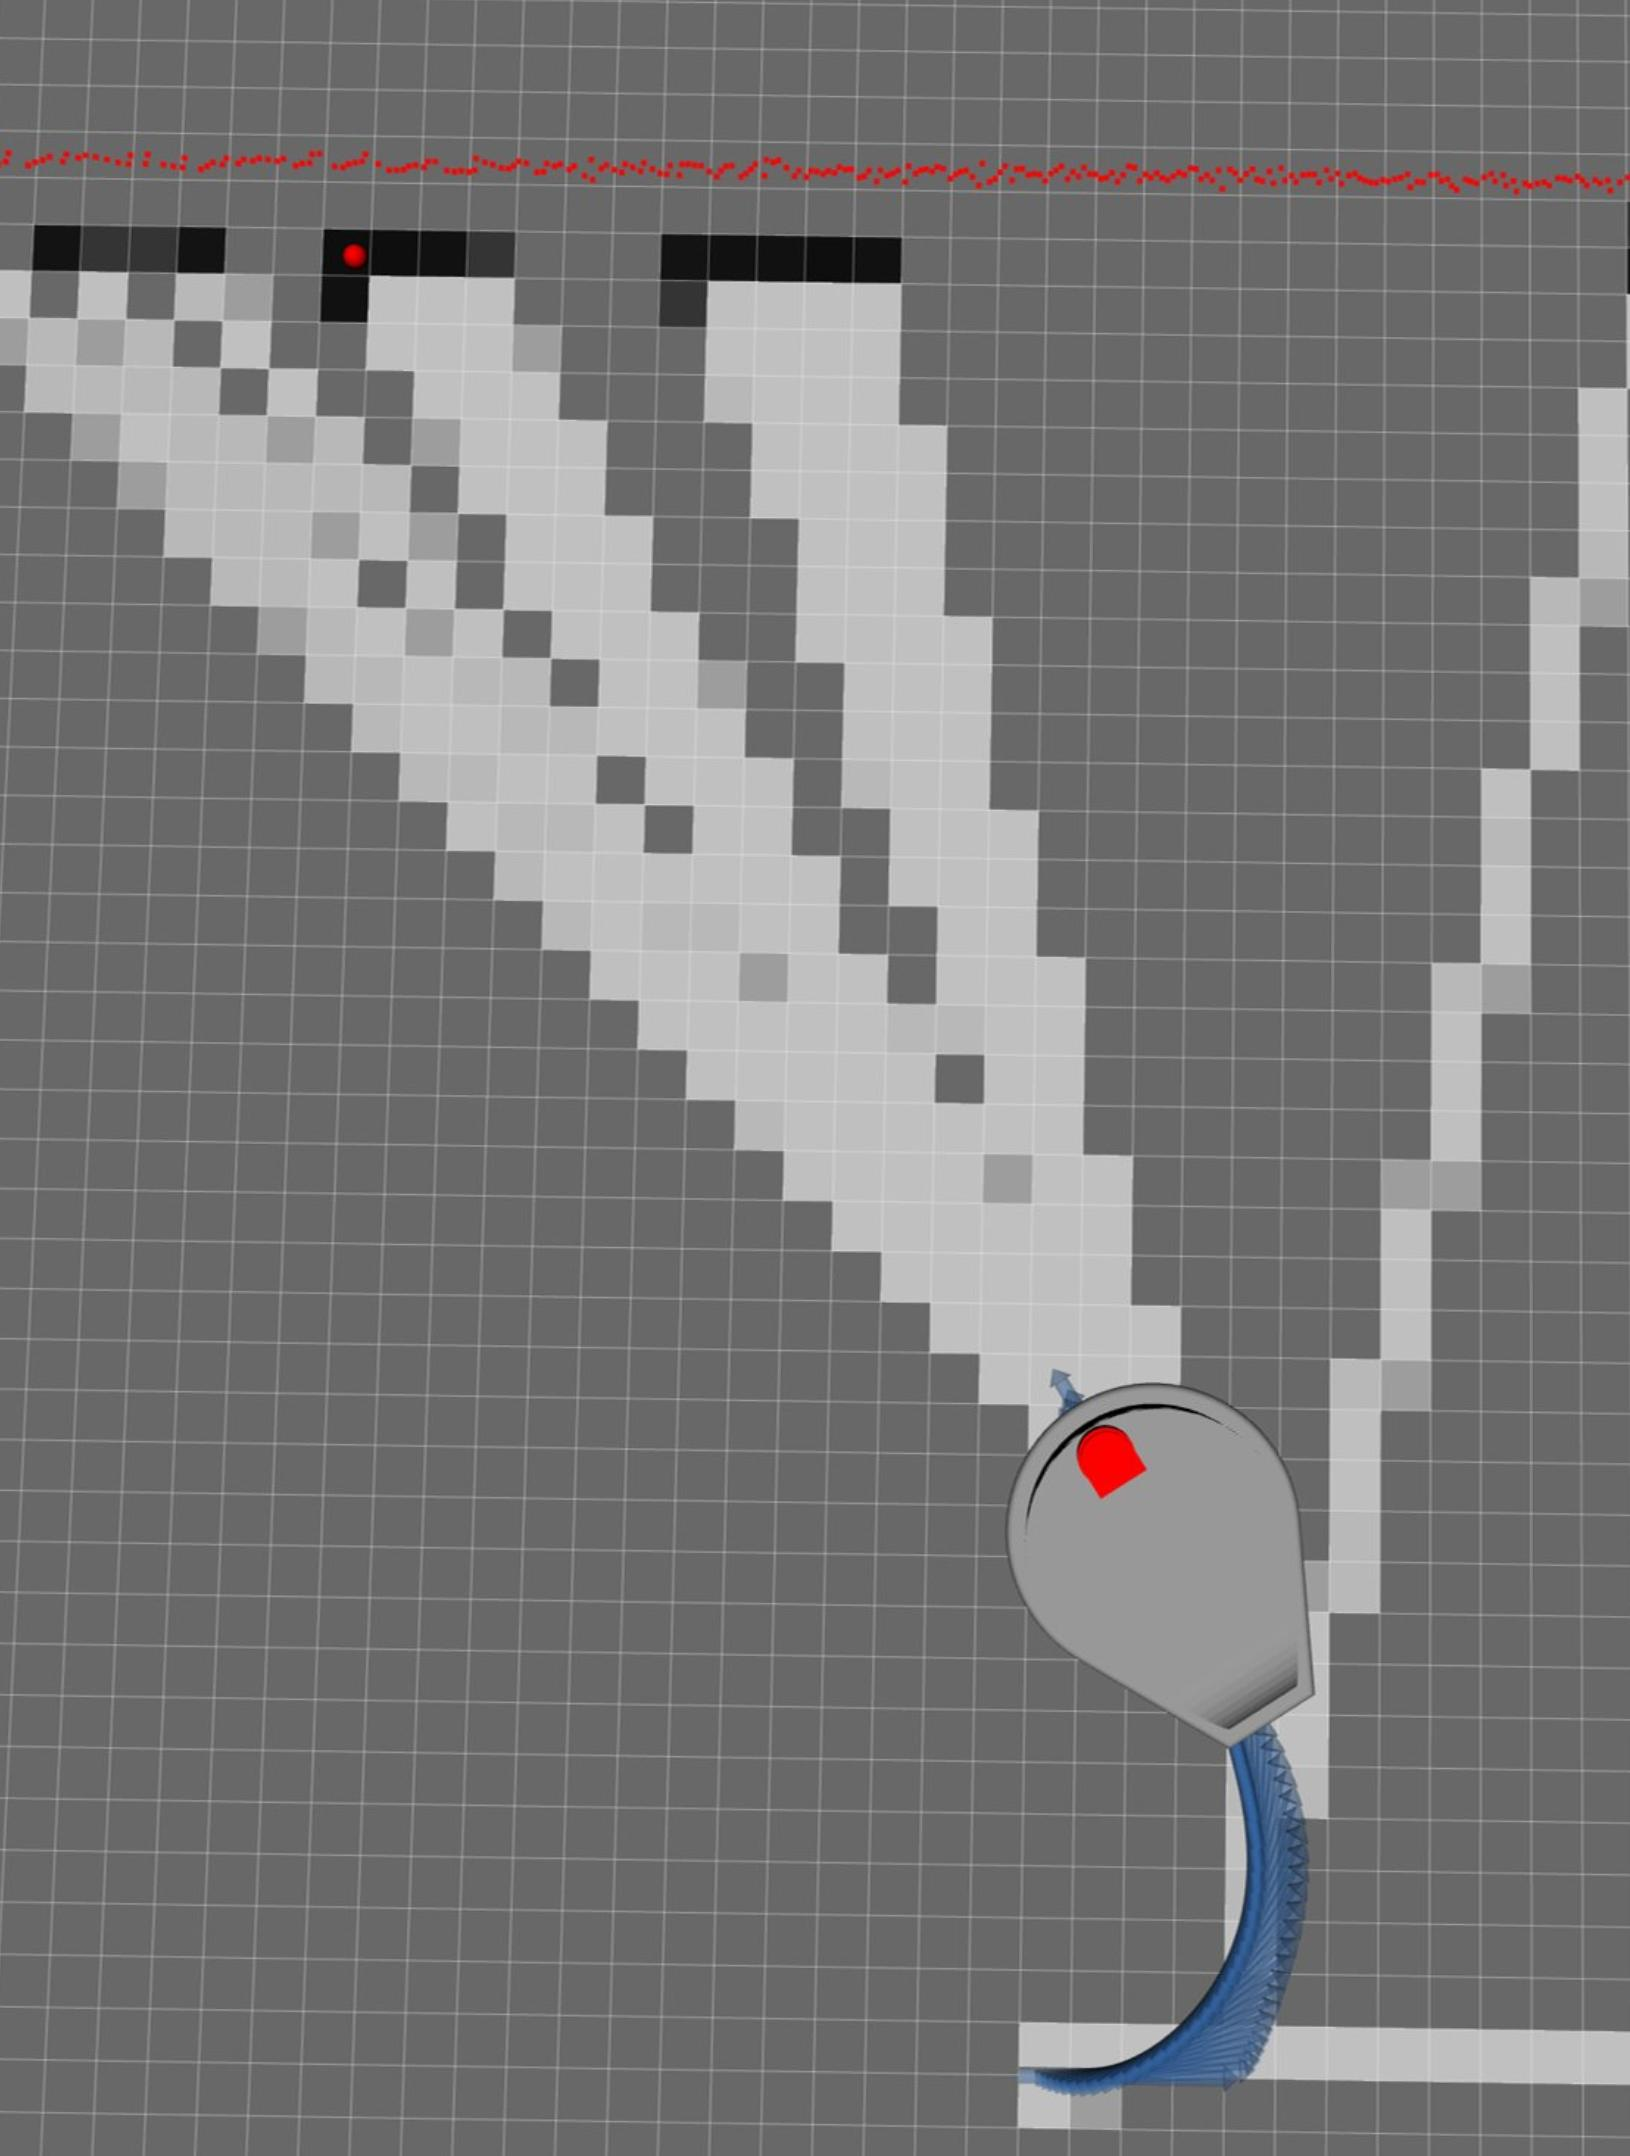
\includegraphics[width=0.3\textwidth]{laser.jpg}
\caption{\label{fig:laser}Cells in the space}
\end{figure}

\begin{itemize}
\item representation: each cell has a value that models occupancy;
\item world is static until new information;
\item pose in the world in know at measurement time;
\item cell is independent;
\end{itemize}

\subsection{Mapping Implementation}
To implement a mapping algorithm of choice and test it in a simulation framework using a virtual SCITOS robot including a laser-range finder as primary sensor.\newline

Two implementations were made for occupancy grid occupancy mapping:
\begin{itemize}
\item using buffer method -- running average of a cell value was updated continuously,
\item using binary Bayesian filter with logarithmic odds form
\end{itemize}

The buffer method was simple implementation to handle the occupancy on a grid. Value of running average of a cell was taken, evaluated and updated. Next implementation used more sophisticated method to store occupancy grid data: the binary Bayesian filter with log odds. \newline

Bayesian filtering is posterior probability distribution of a hypothesis based on a prior knowledge (previous value of a cell) and new observations. We can update the occupancy of the cell using log odds, because it is computationally efficient as it is needed to map value onto range of probabilities between 0 and 1 \cite{test}. Noise from sensor will not affect rapid changes in cell's state. The log odds notation computes the logarithm of the ratio of probabilities, where log odds ratio l is defined as
\[l(x) = \log\left(\frac{p}{1-p}\right)\]
where $p$ represents the probability of an event occurring \cite{lo}. To retrieve $p$ from the log odds ratio following equation is used:
\[p = \frac{1}{1+e^{-\text{log}\left(\frac{p}{1-p}\right)}}\]

To implement cell value update in the map \cite{taltech-bayes} \cite{test} the method results simply to addition of previous cell's value in log odds notion and new measurement:  

\begin{equation}
\label{eq}
\text{l}(p) = \text{inverse sensor model} + \text{previous value} + \text{initial value}
\end{equation}

where $p$ is the probability of occupancy, and the other terms are of logarithmic scale defined as follows: $\text{inverse sensor model}$ is the current sensor measurements transformed into expected probabilities of occupancy, see Figure \ref{fig:ism}; $\text{previous value}$ is the previous occupancy grid estimates; and $\text{initial value}$ is the initial value about the environment before any sensor measurements are taken (which in our case is $\log(0.5)$). \newline

In other words, the equation \ref{eq} shows the probability of occupancy of the cell to the sensor measurements, previous occupancy estimates, and initial assumptions about the environment.

\subsection{Mapping Improvements}

The improvements were made in several areas including:
\begin{itemize}
\item adjusting sensor correctly within the calculations;
\item adding check of invalid sensor measurements;
\item adding logic to update neighboring cells in respect with value $\tau$ marking them as occupied;
\item improving line algorithm.
\end{itemize}

The changes that were added improved the quality of the generated map significantly. The resulting map itself became more accurate in comparison with previous one. The speed of generating the map increased due to optimizations in the line algorithm. Previous line algorithm used linear function  with predefined set of 100 points on the line to update the free space between measurement and the obstacle. New implementation uses Digital Difference Analyzer (DDA) algorithm, which interpolates points based on the difference between the start and end points. Table \ref{tab:widgets} illustrates the difference in the computation in seconds per cycle. \newline


Another algorithm for line points generation was proposed \cite{taltech-line}, but since the optimization using DDA was enough, the Bresenham algorithm can be implemented later in the mapping improvement scope.\newline


\begin{table}
\centering
\label{DDA}
\begin{tabular}{l|l|l}
Function & Linear 100 point approach & DDA point approach \\\hline
Point Processing &  0.457s & 0.009s\\
\end{tabular}
\caption{\label{tab:widgets}Difference between static linear line and DDA points processing algorithms}
\end{table}

Another change of setting neighboring cells occupied had positive effect on the map accuracy. The idea was to find a small value, with notation $\tau$, which in the circle radius it is possible to find points related to the sensor's measurement. The value $\tau$ is experimental, it cannot be too small (otherwise the points  in circle radius would point into the same cell). It cannot be too big, otherwise the result will be incorrect as the cells would be set initially as false-occupied. The factor $\tau$ can be taken into account from Figure \ref{fig:ism}, which should be adjusted according to the expected size of obstacles (e.g. thickness of walls) and the chosen resolution of the map. Demo can be seen here \cite{video-mapping}. Figure \ref{fig:diffence} shows the difference of mapping implementation improvements, the walls and space is much more accurate on the right side, where improvements have been added.

\begin{figure}
\centering
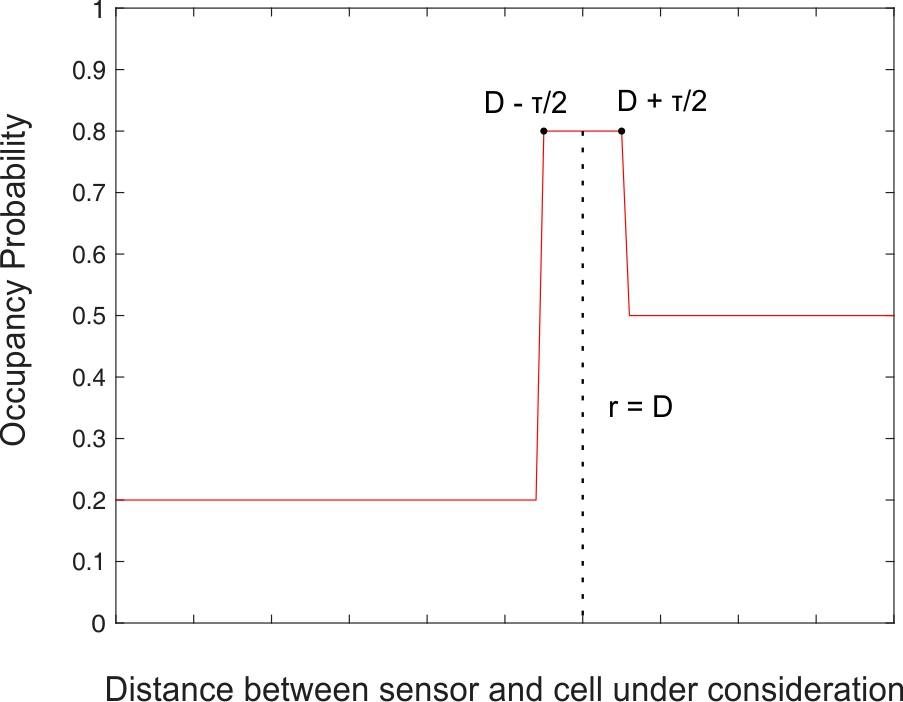
\includegraphics[width=0.5\textwidth]{ism.jpg}
\caption{\label{fig:ism}Inverse Sensor Model \cite{taltech-bayes}}
\end{figure}

\begin{figure}
\centering
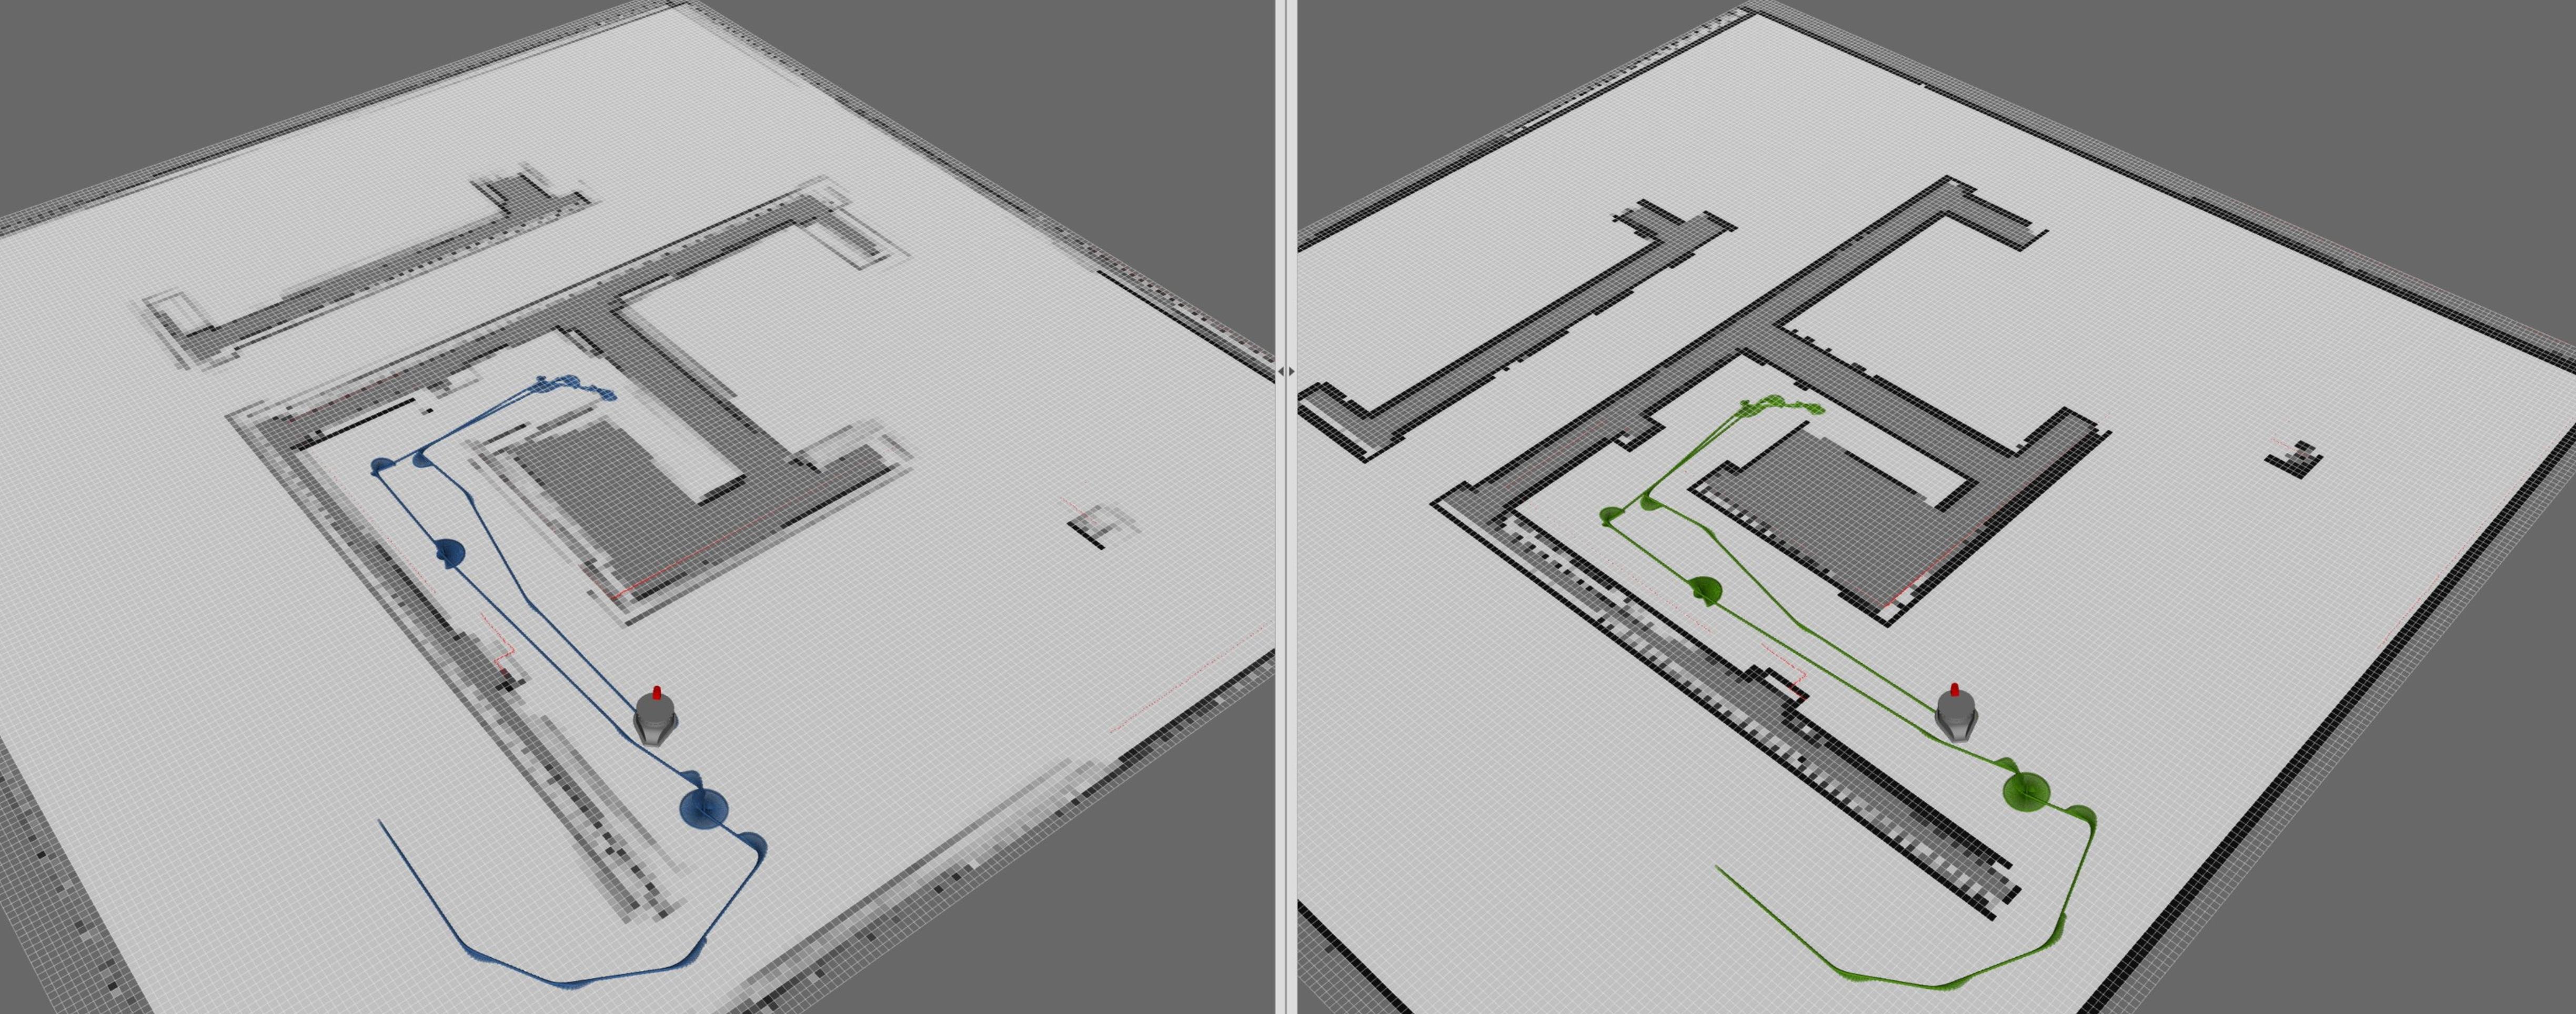
\includegraphics[width=1.0\textwidth]{difference.jpg}
\caption{\label{fig:diffence}Mapping difference using improved mapping implementation \cite{video-mapping}}
\end{figure}


\bibliographystyle{alpha}
\bibliography{sample}

\end{document}